\documentclass[9pt,twocolumn,twoside]{pnas-new}
\usepackage[T1]{fontenc}
\templatetype{pnasresearcharticle}
\articletype{Social Sciences}

% The figures and text should remain readable at the template's native size.
\setboolean{displaywatermark}{false}

% The course report has no assigned journal issue or article number.
\fancyhead{}
\fancypagestyle{firststyle}{%
  \fancyhead{}
  \fancyfoot[L]{\footerfont\textbf{PNAS}}
  \fancyfoot[R]{\footerfont\textbf{\thepage\ of \pageref*{LastPage}}}
}
\fancyfoot[LO]{\footerfont\textbf{PNAS}}

\begin{document}

\title{% Issue 12 draft, 24 November 2026. Title selected and approved by the user.
% Body only: include inside the template's title command.
Does age matter? Premier League entry and changes in Guardian coverage around football signings
}
\author[a,1]{Victor Bohart}
\author[b,1]{Philip Nukunu Fu}
\affil[a]{DTU Management}
\affil[b]{DTU Compute}
\leadauthor{Bohart}
\authorcontributions{% Issue 12, 24 November 2026. User-confirmed equal contributions (50/50).
% Body only: include in the template's author-contributions command.
Victor Bohart and Philip Nukunu Fu contributed equally to this work.
}
\correspondingauthor{{\raggedright
  \textsuperscript{1}Corresponding authors\par
  Victor Bohart, \href{mailto:s230654@dtu.dk}{s230654@dtu.dk}\par
  Philip Nukunu Fu, \href{mailto:s260114@student.dtu.dk}{s260114@student.dtu.dk}\par
}}
\keywords{football transfers $|$ network science $|$ sentiment analysis}
\significancestatement{% Issue 12 draft, 24 November 2026. Revised Significance Statement approved.
% Body only: include in the template's Significance Statement command.
Recruitment records and newspaper coverage offer different perspectives on age in professional football. Older-player transfers had a lower observed Premier League entry rate, although the statistical evidence was limited; in a separate Guardian sample, older signings received more coverage but showed no clear difference in tone changes. More articles about older signings do not necessarily mean more negative coverage, and the lower observed entry rate does not establish that age itself restricted entry into the Premier League.
}

\begin{abstract}
% Issue 12 draft, 24 November 2026. Abstract approved by the user.
% Body only: include inside the template's abstract command/environment.
% 150 words by whitespace count after LaTeX symbol/percent normalization.
How does player age relate to Premier League entry and newspaper coverage around signings? We analysed 16,636 eligible transfers in recorded seasons 2012/13--2024/25 as a directed network and compared entry rates for players aged 30+ and under 30. Older-player transfers entered less often (12.14\% versus 14.56\%), with limited evidence against a null model that shuffled age labels within origin club and recorded season (one-sided p = 0.098). In a separate Guardian sample of 1,332 selected signings, older signings received more coverage. Sentiment analysis retained 820 sufficiently covered signings and compared four instruments against 196 human-labelled sentences. RoBERTa showed the strongest observed rank agreement ($\rho = 0.52$). Its older-minus-younger difference in before-to-after tone changes was +0.0060 (two-sided p = 0.7558), providing no clear evidence of different changes, with limited sensitivity to smaller differences. These findings describe recruitment and selected published language without establishing causal age effects or that coverage influences recruitment.

\end{abstract}

\maketitle
\thispagestyle{firststyle}
{\setlength{\hsize}{1.35\linewidth}\abscontent\par}

\Firstpage
% Issue 12 draft, 24 November 2026. All three Introduction paragraphs approved.
% Recruitment paragraph uses the previously agreed CIES wording.
% Final question/design/contribution paragraph: approved by the user.
% Total Introduction allowance: 0.40 pages; compiled fit remains for Issues 13--14.
\section*{Introduction}

Previous research has documented age differences in football recruitment. A 2022 CIES report found that 10.6\% of externally recruited players in Premier League squads had joined their club at age 30 or older \cite{poli2022recruitment}. In this study, we compare Premier League joining rates among eligible recorded transfers involving players aged 30+ and those under 30.

Previous research has applied sentiment analysis to football coverage from multiple newspaper sources, including the Guardian \cite{dotgrau2019representation}. Monsees (2024) found that German and Swedish newspapers constructed football talent around similar themes, including age, but gave these themes different meanings across cultural contexts \cite{monsees2024talent}. These findings motivate interpreting football coverage in its editorial, linguistic and cultural context.

We ask: \textit{How does entry into the Premier League differ by player age, and how does the tone of Guardian coverage before and after Premier League signings differ by age?} We describe eligible transfers as a network and compare Premier League joining rates for players aged 30+ and under 30. In a separate sample of selected Premier League signings, we compare Guardian sentence sentiment before and after each move to ask whether coverage tone changes differently for older and younger players. To assess the performance of the sentiment models, we compared their scores with manual labels for the same Guardian sentences. One author judged each sentence in the comparison as positive, negative or neutral, providing a human reference for the evaluation. The selected sentences from these articles form the corpus for the sentiment analysis. To describe its vocabulary, we tokenize the sentences and examine which tokens occur most often and how their frequencies vary by rank.

\setlength{\columnwidth}{.3\textwidth}
\Endparasplit

% Include with % Include with % Include with \input{figure_floats} from a PNAS manuscript in paper_simple.
% Plot PDFs contain no manuscript captions; all caption prose is typeset here.
\begin{figure*}[!t]
  \centering
  \includegraphics[trim=8bp 30bp 5bp 10bp,clip,width=0.91\textwidth]{../output/backbone_h1_findings/combined_before_rotation_2026-11-24.pdf}
  \caption{\textbf{Transfer-network structure and Premier League entry by age, recorded seasons 2012/13--2024/25.} Both panels use the same sample of 16,636 eligible transfers involving 4,602 players. \textbf{(a)} The directed disparity backbone at $\alpha = 0.20$ retains 383 clubs and 1,396 routes carrying 5,271 transfers (31.7\% of the sample). Routes are retained when their disparity score is below $\alpha$ at either eligible endpoint. This is an exploratory local filter. Colours and shapes identify five Louvain communities. Each community is named after its member club with the highest total degree before disparity filtering. Arrows point from origin to destination, and line width increases with transfer count. Node area increases with the square root of each club's total incoming and outgoing transfer count before filtering. The network pools both age groups and includes Premier League and other destinations. \textbf{(b)} Using the full sample, Premier League joining rates were 12.14\% for transfers involving players aged 30+ (129/1,063) and 14.56\% for those under 30 (2,267/15,573), an older-minus-younger gap of $-2.42$ percentage points. The histogram shows 999 age-label shuffles within origin club and recorded season, with a mean gap of $-1.31$ points. The legend's $\pm0.83$ denotes one standard deviation of the shuffled gaps; the fitted normal curve is illustrative. The empirical one-sided p-value is 0.098, providing limited evidence against this conditional null.}
  \label{fig:entry-age}
\end{figure*}

\begin{figure*}[!t]
  \centering
  \begin{minipage}[t]{0.47\textwidth}
    \vspace{0pt}
    \centering
    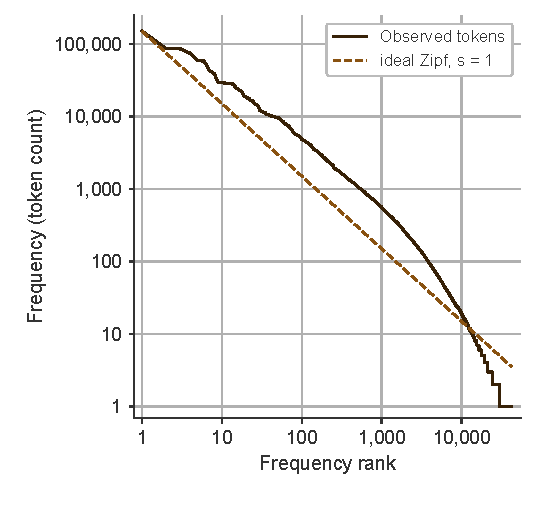
\includegraphics[trim=0bp 13bp 0bp 4bp,clip,width=\linewidth]{../reruns/h1_2012_13-2024_25/output/guardian_text_description_findings/rank_frequency_loglog.pdf}
    \caption{\textbf{Token rank and frequency in the selected Guardian corpus.} Both axes are logarithmic. Counts include stopwords. The ideal Zipf reference divides the most frequent token's count by rank.}
    \label{fig:guardian-rank-frequency}
  \end{minipage}\hfill
  \begin{minipage}[t]{0.50\textwidth}
    \vspace{0pt}
    \centering
    \captionof{table}{Ten most frequent tokens in the selected Guardian corpus, with and without stopwords.}
    \label{tab:guardian-tokens}
    \setlength{\tabcolsep}{3pt}
    \begin{tabular}{@{}rlrrlrr@{}}
      \toprule
      & \multicolumn{3}{c}{With stopwords} & \multicolumn{3}{c}{Without stopwords}\\
      \cmidrule(lr){2-4}\cmidrule(l){5-7}
      Rank & Token & Count & \% & Token & Count & \%\\
      \midrule
      1 & the & 150,246 & 3.9 & season & 17,521 & 0.8\\
      2 & and & 86,037 & 2.2 & \pounds & 15,740 & 0.7\\
      3 & to & 85,471 & 2.2 & m & 14,903 & 0.6\\
      4 & a & 74,360 & 1.9 & city & 11,627 & 0.5\\
      5 & in & 58,569 & 1.5 & united & 11,265 & 0.5\\
      6 & of & 58,167 & 1.5 & chelsea & 10,557 & 0.5\\
      7 & \textquoteright{}s & 42,517 & 1.1 & unknown & 10,439 & 0.4\\
      8 & for & 39,181 & 1.0 & manchester & 10,280 & 0.4\\
      9 & his & 29,501 & 0.8 & form & 10,093 & 0.4\\
      10 & is & 29,321 & 0.8 & injured & 9,960 & 0.4\\
      \bottomrule
    \end{tabular}

    \addtabletext{Percentages use the token total for each ranking (3,870,272 with stopwords and 2,336,122 without stopwords). Both rankings exclude punctuation and whitespace.}
  \end{minipage}
\end{figure*}

% Schedule the monthly plot with the tone-change Results.
\newcommand{\guardianSentimentFigure}{%
\begin{figure*}[!t]
  \centering
  \includegraphics[trim=10bp 8bp 0bp 5bp,clip,width=0.83\textwidth]{../output/h2_monthly_period_means_findings/combined.pdf}
  \caption{\textbf{Guardian sentiment before and after Premier League signings, by age and scoring method.} Panels show RoBERTa (main instrument), VADER, Bing, and Bing excluding 21 football-related words. Higher scores indicate more positive language. Orange identifies signings involving players aged 30+; dark brown identifies those under 30. The sample contains 820 signings (67 older, 753 younger), each with at least five scored sentences in both periods: days $-365$ to $-8$ before signing and +8 to +365 after signing. Liveblogs and match reports are excluded.\endgraf
Curves show monthly sentence scores averaged first within each signing and then across contributing signings, smoothed with a centred three-month moving average separately before and after signing. Monthly membership varies with available coverage. The dashed line marks the signing date. Dots show age-group means of signing-level period means, giving each signing equal weight. Their positions at $-6$ and +6 months are for display; the short horizontal segments are fixed markers. No uncertainty intervals are shown. These period means are calculated separately from the smoothed curves.\endgraf
The main RoBERTa comparison estimates an older-minus-younger difference in before-to-after changes of +0.0060 score units (two-sided p = 0.7558; 5,000 age-label shuffles within signing season). This provides no clear evidence of different changes by age, with limited sensitivity to smaller differences.}
  \label{fig:h2-monthly-tone}
\end{figure*}
}
 from a PNAS manuscript in paper_simple.
% Plot PDFs contain no manuscript captions; all caption prose is typeset here.
\begin{figure*}[!t]
  \centering
  \includegraphics[trim=8bp 30bp 5bp 10bp,clip,width=0.91\textwidth]{../output/backbone_h1_findings/combined_before_rotation_2026-11-24.pdf}
  \caption{\textbf{Transfer-network structure and Premier League entry by age, recorded seasons 2012/13--2024/25.} Both panels use the same sample of 16,636 eligible transfers involving 4,602 players. \textbf{(a)} The directed disparity backbone at $\alpha = 0.20$ retains 383 clubs and 1,396 routes carrying 5,271 transfers (31.7\% of the sample). Routes are retained when their disparity score is below $\alpha$ at either eligible endpoint. This is an exploratory local filter. Colours and shapes identify five Louvain communities. Each community is named after its member club with the highest total degree before disparity filtering. Arrows point from origin to destination, and line width increases with transfer count. Node area increases with the square root of each club's total incoming and outgoing transfer count before filtering. The network pools both age groups and includes Premier League and other destinations. \textbf{(b)} Using the full sample, Premier League joining rates were 12.14\% for transfers involving players aged 30+ (129/1,063) and 14.56\% for those under 30 (2,267/15,573), an older-minus-younger gap of $-2.42$ percentage points. The histogram shows 999 age-label shuffles within origin club and recorded season, with a mean gap of $-1.31$ points. The legend's $\pm0.83$ denotes one standard deviation of the shuffled gaps; the fitted normal curve is illustrative. The empirical one-sided p-value is 0.098, providing limited evidence against this conditional null.}
  \label{fig:entry-age}
\end{figure*}

\begin{figure*}[!t]
  \centering
  \begin{minipage}[t]{0.47\textwidth}
    \vspace{0pt}
    \centering
    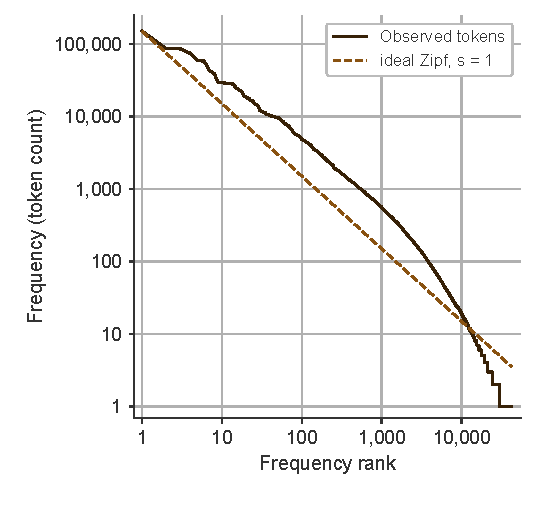
\includegraphics[trim=0bp 13bp 0bp 4bp,clip,width=\linewidth]{../reruns/h1_2012_13-2024_25/output/guardian_text_description_findings/rank_frequency_loglog.pdf}
    \caption{\textbf{Token rank and frequency in the selected Guardian corpus.} Both axes are logarithmic. Counts include stopwords. The ideal Zipf reference divides the most frequent token's count by rank.}
    \label{fig:guardian-rank-frequency}
  \end{minipage}\hfill
  \begin{minipage}[t]{0.50\textwidth}
    \vspace{0pt}
    \centering
    \captionof{table}{Ten most frequent tokens in the selected Guardian corpus, with and without stopwords.}
    \label{tab:guardian-tokens}
    \setlength{\tabcolsep}{3pt}
    \begin{tabular}{@{}rlrrlrr@{}}
      \toprule
      & \multicolumn{3}{c}{With stopwords} & \multicolumn{3}{c}{Without stopwords}\\
      \cmidrule(lr){2-4}\cmidrule(l){5-7}
      Rank & Token & Count & \% & Token & Count & \%\\
      \midrule
      1 & the & 150,246 & 3.9 & season & 17,521 & 0.8\\
      2 & and & 86,037 & 2.2 & \pounds & 15,740 & 0.7\\
      3 & to & 85,471 & 2.2 & m & 14,903 & 0.6\\
      4 & a & 74,360 & 1.9 & city & 11,627 & 0.5\\
      5 & in & 58,569 & 1.5 & united & 11,265 & 0.5\\
      6 & of & 58,167 & 1.5 & chelsea & 10,557 & 0.5\\
      7 & \textquoteright{}s & 42,517 & 1.1 & unknown & 10,439 & 0.4\\
      8 & for & 39,181 & 1.0 & manchester & 10,280 & 0.4\\
      9 & his & 29,501 & 0.8 & form & 10,093 & 0.4\\
      10 & is & 29,321 & 0.8 & injured & 9,960 & 0.4\\
      \bottomrule
    \end{tabular}

    \addtabletext{Percentages use the token total for each ranking (3,870,272 with stopwords and 2,336,122 without stopwords). Both rankings exclude punctuation and whitespace.}
  \end{minipage}
\end{figure*}

% Schedule the monthly plot with the tone-change Results.
\newcommand{\guardianSentimentFigure}{%
\begin{figure*}[!t]
  \centering
  \includegraphics[trim=10bp 8bp 0bp 5bp,clip,width=0.83\textwidth]{../output/h2_monthly_period_means_findings/combined.pdf}
  \caption{\textbf{Guardian sentiment before and after Premier League signings, by age and scoring method.} Panels show RoBERTa (main instrument), VADER, Bing, and Bing excluding 21 football-related words. Higher scores indicate more positive language. Orange identifies signings involving players aged 30+; dark brown identifies those under 30. The sample contains 820 signings (67 older, 753 younger), each with at least five scored sentences in both periods: days $-365$ to $-8$ before signing and +8 to +365 after signing. Liveblogs and match reports are excluded.\endgraf
Curves show monthly sentence scores averaged first within each signing and then across contributing signings, smoothed with a centred three-month moving average separately before and after signing. Monthly membership varies with available coverage. The dashed line marks the signing date. Dots show age-group means of signing-level period means, giving each signing equal weight. Their positions at $-6$ and +6 months are for display; the short horizontal segments are fixed markers. No uncertainty intervals are shown. These period means are calculated separately from the smoothed curves.\endgraf
The main RoBERTa comparison estimates an older-minus-younger difference in before-to-after changes of +0.0060 score units (two-sided p = 0.7558; 5,000 age-label shuffles within signing season). This provides no clear evidence of different changes by age, with limited sensitivity to smaller differences.}
  \label{fig:h2-monthly-tone}
\end{figure*}
}
 from a PNAS manuscript in paper_simple.
% Plot PDFs contain no manuscript captions; all caption prose is typeset here.
\begin{figure*}[!t]
  \centering
  \includegraphics[trim=8bp 30bp 5bp 10bp,clip,width=0.91\textwidth]{../output/backbone_h1_findings/combined_before_rotation_2026-11-24.pdf}
  \caption{\textbf{Transfer-network structure and Premier League entry by age, recorded seasons 2012/13--2024/25.} Both panels use the same sample of 16,636 eligible transfers involving 4,602 players. \textbf{(a)} The directed disparity backbone at $\alpha = 0.20$ retains 383 clubs and 1,396 routes carrying 5,271 transfers (31.7\% of the sample). Routes are retained when their disparity score is below $\alpha$ at either eligible endpoint. This is an exploratory local filter. Colours and shapes identify five Louvain communities. Each community is named after its member club with the highest total degree before disparity filtering. Arrows point from origin to destination, and line width increases with transfer count. Node area increases with the square root of each club's total incoming and outgoing transfer count before filtering. The network pools both age groups and includes Premier League and other destinations. \textbf{(b)} Using the full sample, Premier League joining rates were 12.14\% for transfers involving players aged 30+ (129/1,063) and 14.56\% for those under 30 (2,267/15,573), an older-minus-younger gap of $-2.42$ percentage points. The histogram shows 999 age-label shuffles within origin club and recorded season, with a mean gap of $-1.31$ points. The legend's $\pm0.83$ denotes one standard deviation of the shuffled gaps; the fitted normal curve is illustrative. The empirical one-sided p-value is 0.098, providing limited evidence against this conditional null.}
  \label{fig:entry-age}
\end{figure*}

\begin{figure*}[!t]
  \centering
  \begin{minipage}[t]{0.47\textwidth}
    \vspace{0pt}
    \centering
    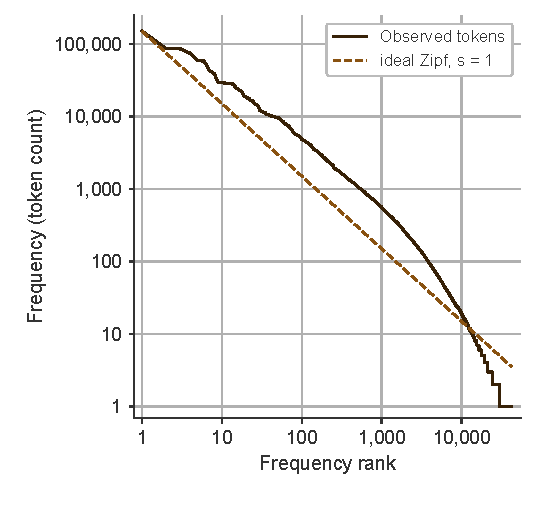
\includegraphics[trim=0bp 13bp 0bp 4bp,clip,width=\linewidth]{../reruns/h1_2012_13-2024_25/output/guardian_text_description_findings/rank_frequency_loglog.pdf}
    \caption{\textbf{Token rank and frequency in the selected Guardian corpus.} Both axes are logarithmic. Counts include stopwords. The ideal Zipf reference divides the most frequent token's count by rank.}
    \label{fig:guardian-rank-frequency}
  \end{minipage}\hfill
  \begin{minipage}[t]{0.50\textwidth}
    \vspace{0pt}
    \centering
    \captionof{table}{Ten most frequent tokens in the selected Guardian corpus, with and without stopwords.}
    \label{tab:guardian-tokens}
    \setlength{\tabcolsep}{3pt}
    \begin{tabular}{@{}rlrrlrr@{}}
      \toprule
      & \multicolumn{3}{c}{With stopwords} & \multicolumn{3}{c}{Without stopwords}\\
      \cmidrule(lr){2-4}\cmidrule(l){5-7}
      Rank & Token & Count & \% & Token & Count & \%\\
      \midrule
      1 & the & 150,246 & 3.9 & season & 17,521 & 0.8\\
      2 & and & 86,037 & 2.2 & \pounds & 15,740 & 0.7\\
      3 & to & 85,471 & 2.2 & m & 14,903 & 0.6\\
      4 & a & 74,360 & 1.9 & city & 11,627 & 0.5\\
      5 & in & 58,569 & 1.5 & united & 11,265 & 0.5\\
      6 & of & 58,167 & 1.5 & chelsea & 10,557 & 0.5\\
      7 & \textquoteright{}s & 42,517 & 1.1 & unknown & 10,439 & 0.4\\
      8 & for & 39,181 & 1.0 & manchester & 10,280 & 0.4\\
      9 & his & 29,501 & 0.8 & form & 10,093 & 0.4\\
      10 & is & 29,321 & 0.8 & injured & 9,960 & 0.4\\
      \bottomrule
    \end{tabular}

    \addtabletext{Percentages use the token total for each ranking (3,870,272 with stopwords and 2,336,122 without stopwords). Both rankings exclude punctuation and whitespace.}
  \end{minipage}
\end{figure*}

% Schedule the monthly plot with the tone-change Results.
\newcommand{\guardianSentimentFigure}{%
\begin{figure*}[!t]
  \centering
  \includegraphics[trim=10bp 8bp 0bp 5bp,clip,width=0.83\textwidth]{../output/h2_monthly_period_means_findings/combined.pdf}
  \caption{\textbf{Guardian sentiment before and after Premier League signings, by age and scoring method.} Panels show RoBERTa (main instrument), VADER, Bing, and Bing excluding 21 football-related words. Higher scores indicate more positive language. Orange identifies signings involving players aged 30+; dark brown identifies those under 30. The sample contains 820 signings (67 older, 753 younger), each with at least five scored sentences in both periods: days $-365$ to $-8$ before signing and +8 to +365 after signing. Liveblogs and match reports are excluded.\endgraf
Curves show monthly sentence scores averaged first within each signing and then across contributing signings, smoothed with a centred three-month moving average separately before and after signing. Monthly membership varies with available coverage. The dashed line marks the signing date. Dots show age-group means of signing-level period means, giving each signing equal weight. Their positions at $-6$ and +6 months are for display; the short horizontal segments are fixed markers. No uncertainty intervals are shown. These period means are calculated separately from the smoothed curves.\endgraf
The main RoBERTa comparison estimates an older-minus-younger difference in before-to-after changes of +0.0060 score units (two-sided p = 0.7558; 5,000 age-label shuffles within signing season). This provides no clear evidence of different changes by age, with limited sensitivity to smaller differences.}
  \label{fig:h2-monthly-tone}
\end{figure*}
}

% Issue 12 draft, 24 November 2026. Review/source map: Issue 12.
% Issue 9.1: corpus-description addition approved; existing Results preserved.
% Transfer-network structure: approved by the user, including tone/explanation.
% Premier League entry by age: approved by the user.
% Guardian coverage volume: approved, with the short zero-coverage clarification.
% Measuring tone in football writing: approved, including revised averaging text.
% Changes in Guardian tone by age: approved by the user.
% All five Results subsections are approved; compiled fit remains for Issues 13--14.
% Template assembly, bibliography integration and compilation: Issues 13--14.
\section*{Results}

\subsection*{Transfer-network structure}

We first represented eligible transfers as a directed network, with clubs as nodes and origin--destination routes weighted by the number of transfers. The 16,636 transfers involving 4,602 players in recorded seasons 2012/13--2024/25 connected 1,157 clubs through 11,016 routes.

Figure~\ref{fig:entry-age}(a) shows a filtered view of this network using a disparity cutoff of $\alpha = 0.20$ \cite{serrano2009multiscale}. The backbone retained 383 clubs and 1,396 routes carrying 5,271 transfers (31.7\% of the sample). Colours and shapes identify five communities found by directed Louvain on the full network \cite{blondel2008louvain,dugue2015directed}. This view pools both age groups and includes Premier League and other destinations. The entry-by-age comparison below uses the full transfer sample.

We also explored Leiden, a refinement of the widely used Louvain method that addresses problems with community connectivity \cite{traag2019leiden}. Its original evaluation reported faster runtime than Louvain. Both methods identified five communities in the observed network, with broadly similar club memberships. Modularity was higher in the observed network than in the same randomized network for both Leiden (0.448 versus 0.215) and Louvain (0.446 versus 0.213). By this measure, transfer activity was more strongly concentrated within communities in the observed network.

\subsection*{Premier League entry by age}

We compared the share of eligible transfers entering the Premier League for the two age groups (Figure~\ref{fig:entry-age}(b)). To assess the gap, we shuffled age labels among transfers from the same origin club and recorded season, keeping destinations fixed.

Among eligible recorded transfers in source seasons 2012/13--2024/25, 12.14\% of transfers involving players aged 30+ entered the Premier League, compared with 14.56\% for players under 30 (gap $-2.42$ percentage points). The observed gap was more negative than the mean within-origin-club/season permutation gap ($-1.31$ points), but evidence against this null was limited (one-sided p = 0.098).

Players can make several transfers over their careers, so frequent movers contribute more observations to the main analysis and may disproportionately influence the comparison between age groups. As a sensitivity check, we selected one eligible transfer uniformly at random for each player and repeated the permutation analysis on this fixed sample. This gave every eligible player equal representation, allowing us to examine whether the observed age difference also appeared after removing repeated contributions. In this sample of 4,602 players, joining rates remained lower for transfers involving players aged 30+ (19.52\% versus 21.46\%; gap $-1.94$ percentage points; one-sided p = 0.074). The result is conditional on this one selection and does not assess variation across alternative selections.

\subsection*{Guardian coverage volume}

We examined Guardian coverage in a separate sample of 1,332 selected Premier League signings. The collected coverage included 43,924 distinct articles before sentiment filters were applied. To describe attention around each signing, we counted distinct articles naming the player before and after the move, including all article types.

Older signings received more Guardian coverage in both periods. The median number of distinct articles per signing was 27.5 for players aged 30+ versus 12 for those under 30 before signing, and 47.5 versus 35 after signing. Counts include signings with no recorded coverage.

\subsection*{Measuring tone in football writing}

For the tone comparison, a signing needed at least five scored sentences both before and after the move, after excluding liveblogs and match reports. This left 820 signings: 67 involving players aged 30+ and 753 involving younger players.

The selected corpus comprised 99,976 linked sentence records, containing 3.87 million tokens and 42,779 token types, of which 13,022 were hapax tokens. Table~\ref{tab:guardian-tokens} lists the ten most frequent tokens in each ranking, with and without stopwords. After removing stopwords, frequent tokens included ``season'', club-name components such as ``city'' and ``united'', and ``form'', ``injured'' and ``unknown''. Figure~\ref{fig:guardian-rank-frequency} shows frequency rank and raw counts with stopwords on logarithmic axes, with an ideal Zipf reference ($s = 1$) anchored to the most frequent token. Counts lay above this reference for many common tokens and below it for the rarest tokens. These counts partly describe the vocabulary of the selected corpus. The following analysis examines the tone of the sentences.

We applied four scoring methods to player-linked sentences, including quotations: RoBERTa \cite{liu2019roberta,loureiro2022timelms,camachocollados2022tweetnlp,cardiffnlp2022checkpoint}, VADER \cite{hutto2014vader}, the Bing opinion lexicon \cite{hu2004mining}, and Bing excluding 21 football-related words. Higher scores indicate more positive language. For the overall before--after comparison, we averaged all available sentence scores for each signing separately before and after the move. The monthly curves in Figure~\ref{fig:h2-monthly-tone} were calculated separately, using sentence scores from each month. These scores describe how the selected published sentences read; they do not directly identify the journalist's attitude toward the player.

To check the scores against human judgments, one author labelled 200 sentences. Four wrong-person matches were excluded, leaving 196 evaluable sentences.

Table~\ref{tab:validation} checks three aspects of the sentence scores. The human labels were ordered from negative to neutral to positive, with all sentences in each category sharing a rank. Spearman's $\rho$ compares those category ranks with the ranks of each model's numerical scores. A positive $\rho$ indicates that the model's ranking tended to agree with the order of the three categories. Correct sign measures whether scores are above zero for human-positive sentences and below zero for human-negative sentences, excluding human-neutral cases. Three-class accuracy measures exact agreement with positive, neutral or negative labels across all sentences. RoBERTa had the strongest observed rank agreement ($\rho = 0.52$, 95\% bootstrap interval 0.38--0.63) and the correct sign for 70 of 85 positive or negative sentences (82\%). Its three-class predictions matched 98 of 196 labels (50\%), showing the difficulty of distinguishing neutral language. These checks support using RoBERTa as a useful but imperfect measure; the 14 older-player sentences leave age-specific comparability uncertain.

% Approved Table 1 values, caption and note, 24 November 2026.
% Native LaTeX transcription for Issue 12; compiled layout checked in Issues 13--14.
\begin{table}[tbhp]
\centering
\small
\setlength{\tabcolsep}{4.5pt}
\caption{Agreement of four sentiment instruments with human judgments of Guardian sentences.}
\label{tab:validation}
\begin{tabular}{lccc}
\toprule
Instrument & $\rho$ (95\% CI) & Sign right & 3-class accuracy \\
\midrule
RoBERTa & 0.52 (0.38, 0.63) & 82\% & 50\% \\
VADER & 0.33 (0.21, 0.45) & 68\% & 42\% \\
Bing & 0.36 (0.22, 0.47) & 59\% & 51\% \\
Bing, no football words & 0.36 (0.23, 0.49) & 58\% & 53\% \\
\bottomrule
\end{tabular}
\addtabletext{Results use 196 hand-labelled sentences after excluding four wrong-person matches. Spearman's $\rho$ measures whether sentences judged more positive receive higher scores; 95\% confidence intervals use 2,000 sentence bootstrap resamples. Correct sign is the percentage of the 85 human-positive or human-negative sentences whose score has the corresponding sign. Three-class accuracy is the percentage of all 196 sentences classified correctly as positive, neutral or negative. Neutral scores fall within $\pm0.05$ for RoBERTa and VADER and equal zero for both Bing variants. Only 14 sentences concern players aged 30+, leaving age-specific validity uncertain.}
\end{table}


\guardianSentimentFigure
\subsection*{Changes in Guardian tone by age}

Figure~\ref{fig:h2-monthly-tone} shows monthly mean sentence sentiment for older and younger signings, separately for RoBERTa, VADER and the two Bing variants. For each signing, we first averaged the sentiment scores of the sentences published in a given month. We then averaged these monthly values separately for older and younger signings. Only signings with sentences in a month contributed to that month's average. The curves show these monthly group means smoothed with a centred three-month moving average, separately before and after signing.

First, we calculated one tone change per signing by subtracting its mean sentiment score before the move from its mean score after the move. We averaged these changes within each age group, giving every signing equal weight. With RoBERTa, the mean change was $-0.0076$ for the 30+ group and $-0.0137$ for the under-30 group. Subtracting the younger group's mean change from the older group's, using unrounded values, gave a gap of +0.0060 score units.

We kept each signing's tone change fixed and shuffled the age-group labels within each season 5,000 times, recalculating the gap after each shuffle. We found no clear evidence that sentiment changed differently for older and younger signings. VADER and both Bing variants also provided no clear evidence of different changes.

\subsection*{Sub-analysis of the transfer network}

During the network analysis, we also examined which club pairs accounted for unusually many transfers among the 2,396 Premier League arrivals. The exploratory screen selected 217 recurring routes, each with at least two recorded transfers, accounting for 626 transfers (Figure~\ref{fig:feeder-routes}). Girona to Manchester City was the busiest transfer pair, with 15 recorded transfers over the study period. We calculated an expected count for that route in each season, keeping fixed how many transfers each origin club sent to the Premier League and how many each destination club received. Adding those seasonal expectations gave an expected total of 1.8 transfers across the full 2012/13--2024/25 period.

We found that some high-volume transfer pairs shared a common equity investor. The 17 transfer pairs in the joint-ownership group had a median of four transfers. In comparison, the remaining 200 transfer pairs had a median of two (Figure~\ref{fig:feeder-routes}b).

\begin{figure*}[!t]
  \centering
  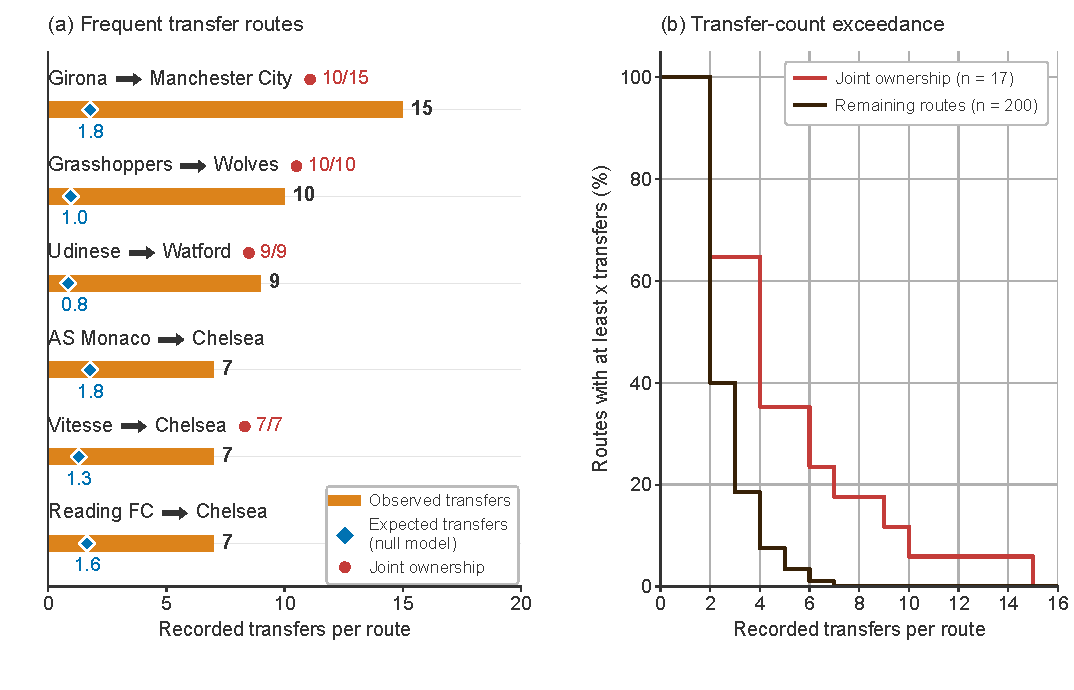
\includegraphics[trim=16bp 20bp 0bp 3bp,clip,width=0.80\textwidth]{../reruns/h1_2012_13-2024_25/output/premier_league_feeder_findings_three_panel.pdf}
  \caption{\textbf{Recurring transfer routes into the Premier League.} \textbf{(a)} The six screened transfer pairs with at least seven recorded transfers among 2,396 arrivals in recorded seasons 2012/13--2024/25. Bars show observed counts and diamonds show expectations under the seasonal destination shuffle. For Girona and Udinese, the red fractions show how many of each route's transfers occurred during documented joint ownership. \textbf{(b)} The exceedance curves show the percentage of routes in each group with at least a given number of recorded transfers.}
  \label{fig:feeder-routes}
\end{figure*}

% Issue 12 draft, 24 November 2026. All four Discussion paragraphs approved.
% Issue 9.1: Zipf explanation approved after wording clarification.
% Includes the approved, explicitly labelled invented sentiment illustration.
% Total Discussion allowance: 0.55 pages; compiled fit remains for Issues 13--14.
\section*{Discussion}

Older-player transfers had a lower observed Premier League joining rate, with limited evidence against the origin-club/season null. In separate Guardian samples, older signings received more coverage, while tone changes showed no clear age difference. Greater coverage describes more attention, without establishing more negative treatment. These separate samples do not establish that press tone and recruitment decisions influence one another.

The lower observed entry rate does not establish that age itself restricted entry. Differences in player characteristics or preferences could contribute, but these explanations were not tested. Because the data record completed moves rather than offers and rejections, they cannot identify recruitment motives.

The sentiment comparison also depends on which signings had sufficient qualifying text. The filters retained 67 of 88 older signings and 753 of 1,244 younger signings, limiting generalisation to all selected signings. Player prominence and the mix of performances, topics and quoted voices could affect the measured tone, but their contributions were not tested. Some rare words may appear only once because our sample contains a limited amount of text. How we split expressions into tokens, and the repeated use of club names and injury updates, may also affect the frequency pattern. We did not test whether these factors explain why the vocabulary in our text analysis diverges from the ideal Zipf law in this log--log comparison of frequency rank and raw token frequency. RoBERTa scores the whole sentence without being told which player to evaluate. Its score may therefore reflect praise or criticism of another person mentioned in the same sentence \cite{hamborg2021news}. For an \textit{invented illustration}, consider ``Smith watched as Jones delivered an outstanding performance.'' This sentence names Smith but praises Jones, so a positive sentence score could enter Smith's coverage average without expressing praise for Smith. Validation by one annotator, including only 14 older-player sentences, leaves age-specific validity uncertain. Smaller differences in tone change remain possible; the inconclusive comparison does not establish equal changes.

Some players appear more than once, and the same article can contribute to several signings. The age-label shuffles may not fully account for these links between observations. This limits how confidently we can interpret the p-values \cite{hemerik2018exact,winkler2015multilevel}. The text findings describe selected English-language Guardian coverage. Monsees's comparison of German and Swedish newspapers motivates caution about generalising across editorial, linguistic and cultural contexts \cite{monsees2024talent}. Missing original article text and score caches also limit independent reconstruction.

\matmethods{% Issue 12 draft, 24 November 2026. Complete Methods drafting pass approved.
% Issue 9.1: descriptive token/Zipf methods approved; prior prose preserved.
% The three sample paragraphs are the exact previously approved wording.
% Study samples/provenance: approved following the requested detail removals.
% Transfer network/backbone: approved by the user.
% H1 null explanation, assumption, empirical equation and sensitivity: approved.
% Guardian article retrieval/coverage: approved by the user.
% Sentence-selection paragraph: approved with the requested He/His wording.
% Sentiment instruments and validation paragraphs: approved by the user.
% H2 comparison/monthly display: approved with averaging/smoothing/markers preserved.
% Closing code-development statement: approved by the user.
% Template assembly: include inside \matmethods{% Issue 12 draft, 24 November 2026. Complete Methods drafting pass approved.
% Issue 9.1: descriptive token/Zipf methods approved; prior prose preserved.
% The three sample paragraphs are the exact previously approved wording.
% Study samples/provenance: approved following the requested detail removals.
% Transfer network/backbone: approved by the user.
% H1 null explanation, assumption, empirical equation and sensitivity: approved.
% Guardian article retrieval/coverage: approved by the user.
% Sentence-selection paragraph: approved with the requested He/His wording.
% Sentiment instruments and validation paragraphs: approved by the user.
% H2 comparison/monthly display: approved with averaging/smoothing/markers preserved.
% Closing code-development statement: approved by the user.
% Template assembly: include inside \matmethods{% Issue 12 draft, 24 November 2026. Complete Methods drafting pass approved.
% Issue 9.1: descriptive token/Zipf methods approved; prior prose preserved.
% The three sample paragraphs are the exact previously approved wording.
% Study samples/provenance: approved following the requested detail removals.
% Transfer network/backbone: approved by the user.
% H1 null explanation, assumption, empirical equation and sensitivity: approved.
% Guardian article retrieval/coverage: approved by the user.
% Sentence-selection paragraph: approved with the requested He/His wording.
% Sentiment instruments and validation paragraphs: approved by the user.
% H2 comparison/monthly display: approved with averaging/smoothing/markers preserved.
% Closing code-development statement: approved by the user.
% Template assembly: include inside \matmethods{\input{methods}}.
% Total Methods allowance: 1.00 page; compiled fit remains for Issues 13--14.
\subsection*{Study samples and provenance}

We used two separate study samples acquired through different routes. The transfer analysis included 16,636 eligible transfer records involving 4,602 players in recorded source seasons 2012/13--2024/25. Transfers originated at real clubs outside the Premier League under season-specific membership, passed the existing club exclusions, and had at least one endpoint in a top-five league. Of these records, 15,573 involved players under 30 and 1,063 involved players aged 30 or older. Premier League joining rates use all eligible transfers within each age group as their denominators. Network analyses aggregate the same transfer records.

The Guardian analysis used 1,332 selected Premier League signings involving 980 players in July--June seasons 2012/13--2024/25. Signing eligibility required age 18--36 and recorded market value of at least EUR 2 million; same-club moves and heuristic loan returns were excluded, with paid reversals retained. Coverage volume includes all selected signings. Main sentiment analysis retained 820 signings with at least five scored sentences in both the before and after periods, after excluding liveblogs and match reports. Both samples classify age in completed years at the transfer date and compare players aged 30+ with those under 30.

These analyses address age differences in Premier League entry and coverage using separate event populations. The Guardian sample includes signings from within the league and follows different age, value, club and return rules. Its signing metadata is Transfermarkt-derived, while its measured text is from the Guardian. The samples do not follow a shared cohort from recruitment into media coverage.

Transfer and signing metadata were derived from Transfermarkt \cite{transfermarkt_kaggle}. Guardian articles were collected through the Guardian Open Platform \cite{guardian_api}. The transfer analysis used recorded season labels. Guardian signing seasons were assigned from transfer dates using July--June years.

\subsection*{Transfer network and backbone}

We pooled eligible transfers across seasons and age groups into a directed weighted network. Clubs were nodes, and each sending--receiving route was weighted by its transfer count. Communities were identified with directed weighted Louvain at resolution 1 and random seed 2026 \cite{blondel2008louvain,dugue2015directed}. We also explored Leiden on the same graph with the same modularity objective and seed \cite{traag2019leiden}. We generated one randomized network by rewiring routes while preserving each club's number of incoming and outgoing routes, then randomly reassigning the original route weights. We ran both methods on this same network.

For Figure~\ref{fig:entry-age}(a), we applied the directed disparity filter \cite{serrano2009multiscale}. For each route, we examined its share of the sending club's outgoing transfers and the receiving club's incoming transfers. These shares were compared with a uniform random allocation of transfer weight among the corresponding routes. We retained a route if its disparity score was strictly below 0.20 at either club. An outgoing score required more than one outgoing route; an incoming score required more than one incoming route. Community labels were assigned before filtering, and H1 used the full transfer sample.

\subsection*{Entry-rate comparison and player sensitivity}

The H1 null distribution was generated from the full eligible transfer sample, including Premier League and other destinations. We shuffled the 30+/under-30 labels 999 times within origin club and recorded season, keeping destinations and the numbers of older and younger transfers in each club--season group fixed. For each shuffle, we recalculated the older-minus-younger difference in Premier League joining rates, in percentage points, using all eligible transfers in each age group as denominators. The age groups therefore retained their original mix of clubs and seasons, allowing their overall joining rates to remain different after shuffling. The test assumes that age labels are interchangeable among transfers from the same origin club and season under the null.

The empirical one-sided p-value was the fraction of shuffled gaps at or below the observed gap, with one added to both the numerator and denominator \cite{hemerik2018exact,phipson2010permutation}:
\begin{equation}
p_{\mathrm{emp}} =
\frac{1+\text{number of shuffles at least as extreme}}
     {1+\text{number of shuffles}}.
\label{eq:h1-empirical-p}
\end{equation}

For the player sensitivity check, we selected one eligible transfer uniformly at random for each player, without using age or destination to choose it. We held this subset fixed and applied the same within-origin-club/season procedure, again using 999 age-label shuffles. This gave each player equal representation while changing the weighting and composition of transfers. The analysis did not assess variation across alternative selections. Seed 2026 generated separate random streams for the main shuffles, transfer selection and sensitivity shuffles.

\subsection*{Recurring routes into the Premier League}

We counted 2,396 Premier League arrivals from the 16,636 eligible transfers in recorded seasons 2012/13--2024/25 by directed club pair. We shuffled destinations 999 times within each season (seed 2026), preserving each origin and destination total. We retained routes with at least two recorded transfers and an unadjusted upper-tail permutation $p < 0.05$. The joint-ownership group included transfer pairs whose clubs shared an equity investor, plus two pairs included on the basis of family or financial ties.

\subsection*{Guardian articles and coverage volume}

We searched the Guardian Open Platform's football section using player-name variants over the 365 days before and after each signing \cite{guardian_api}. Duplicate article--signing links were removed. When an article was linked to several signings of the same player, we retained the link to the nearest signing date, choosing the earlier signing in a tie. An article could still contribute to signings involving different players.

For coverage volume, we counted distinct article IDs with at least one coded player-name mention for each signing, separately over days $-365$ to $-8$ before signing and $+8$ to $+365$ after signing. We included all article types and all 1,332 selected signings, assigning zero where no qualifying article was recorded. We then calculated median article counts separately for each age group and period. These descriptive counts preceded the sentence-coverage and article-type filters used for sentiment analysis.

\subsection*{Sentence sentiment and validation}

We selected sentences using player-name matching, with rules to reduce confusion between people with similar names. We also retained the immediately following sentence when it began with ``He'' or ``His''. Quotations and brief mentions were retained.

For the corpus description, we selected original sentence records using H2's saved signing membership and article/date filters. We counted lowercase surface tokens with spaCy's English tokenizer after removing punctuation and whitespace, retaining names, numbers, inflections and repeated linked records, and repeated the ranking after excluding English stopwords. We compared ranked counts with $c_1/r$, where $c_1$ is the most frequent token count and $r$ is frequency rank; no exponent was fitted.

Our main instrument was CardiffNLP's \nolinkurl{twitter-roberta-base-sentiment-latest} \cite{liu2019roberta,loureiro2022timelms,camachocollados2022tweetnlp,cardiffnlp2022checkpoint}. It scored each whole sentence as $P(\mathrm{positive})-P(\mathrm{negative})$, truncating inputs at 128 tokens, without a separately specified player target. We also used VADER's compound score \cite{hutto2014vader,vader_documentation} and the Bing opinion lexicon \cite{hu2004mining,textdata_bing_documentation}. Bing scores were positive minus negative word counts divided by their sum, or zero if no lexicon words matched. A second Bing variant excluded 21 football-related words listed in the scoring code. Higher scores indicated more positive language.

One author labelled 200 sentences as positive, neutral, negative or wrong-person matches. Excluding four wrong-person cases left 196 evaluable sentences. We compared scores with ordered human labels using Spearman's $\rho$, checked score signs on the 85 human-positive or human-negative sentences, and assessed exact three-class agreement on all 196 sentences using the neutral thresholds in Table~\ref{tab:validation}. Rank-correlation intervals used the 2.5th and 97.5th percentiles of 2,000 sentence bootstrap resamples (seed 2805). Only 14 evaluated sentences concerned older players, limiting age-specific validation.

\subsection*{Tone changes and monthly display}

For H2, we used the before and after windows defined above, excluded liveblogs and match reports, and required at least five scored sentences in each period. For each instrument, we averaged sentence sentiment scores separately before and after each signing and calculated the after-minus-before change. We then compared mean changes between players aged 30+ and under 30, giving each signing equal weight.

We shuffled age labels 5,000 times within signing season (seed 2805), keeping each signing's tone change fixed. The two-sided empirical p-value was the fraction of shuffled gaps whose absolute value was at least that of the observed older-minus-younger gap, with one added to both the numerator and denominator \cite{hemerik2018exact,phipson2010permutation}. The test assumes that age labels are interchangeable among signings in the same season under the null.

For Figure~\ref{fig:h2-monthly-tone}, we averaged sentence sentiment first within each signing and month, then across contributing signings in each age group. Monthly membership varied with available coverage. We smoothed these group means with a centred three-month moving average separately before and after signing, using two months at the endpoints. Period-mean markers were calculated separately from the curves, using the signing-level period means. Their short horizontal segments are fixed display markers; no uncertainty intervals are shown.

\subsection*{Code development}

The analysis code was developed partly with support from coding agents operating in a terminal, reflecting the course's emphasis on this approach to computational work.
}.
% Total Methods allowance: 1.00 page; compiled fit remains for Issues 13--14.
\subsection*{Study samples and provenance}

We used two separate study samples acquired through different routes. The transfer analysis included 16,636 eligible transfer records involving 4,602 players in recorded source seasons 2012/13--2024/25. Transfers originated at real clubs outside the Premier League under season-specific membership, passed the existing club exclusions, and had at least one endpoint in a top-five league. Of these records, 15,573 involved players under 30 and 1,063 involved players aged 30 or older. Premier League joining rates use all eligible transfers within each age group as their denominators. Network analyses aggregate the same transfer records.

The Guardian analysis used 1,332 selected Premier League signings involving 980 players in July--June seasons 2012/13--2024/25. Signing eligibility required age 18--36 and recorded market value of at least EUR 2 million; same-club moves and heuristic loan returns were excluded, with paid reversals retained. Coverage volume includes all selected signings. Main sentiment analysis retained 820 signings with at least five scored sentences in both the before and after periods, after excluding liveblogs and match reports. Both samples classify age in completed years at the transfer date and compare players aged 30+ with those under 30.

These analyses address age differences in Premier League entry and coverage using separate event populations. The Guardian sample includes signings from within the league and follows different age, value, club and return rules. Its signing metadata is Transfermarkt-derived, while its measured text is from the Guardian. The samples do not follow a shared cohort from recruitment into media coverage.

Transfer and signing metadata were derived from Transfermarkt \cite{transfermarkt_kaggle}. Guardian articles were collected through the Guardian Open Platform \cite{guardian_api}. The transfer analysis used recorded season labels. Guardian signing seasons were assigned from transfer dates using July--June years.

\subsection*{Transfer network and backbone}

We pooled eligible transfers across seasons and age groups into a directed weighted network. Clubs were nodes, and each sending--receiving route was weighted by its transfer count. Communities were identified with directed weighted Louvain at resolution 1 and random seed 2026 \cite{blondel2008louvain,dugue2015directed}. We also explored Leiden on the same graph with the same modularity objective and seed \cite{traag2019leiden}. We generated one randomized network by rewiring routes while preserving each club's number of incoming and outgoing routes, then randomly reassigning the original route weights. We ran both methods on this same network.

For Figure~\ref{fig:entry-age}(a), we applied the directed disparity filter \cite{serrano2009multiscale}. For each route, we examined its share of the sending club's outgoing transfers and the receiving club's incoming transfers. These shares were compared with a uniform random allocation of transfer weight among the corresponding routes. We retained a route if its disparity score was strictly below 0.20 at either club. An outgoing score required more than one outgoing route; an incoming score required more than one incoming route. Community labels were assigned before filtering, and H1 used the full transfer sample.

\subsection*{Entry-rate comparison and player sensitivity}

The H1 null distribution was generated from the full eligible transfer sample, including Premier League and other destinations. We shuffled the 30+/under-30 labels 999 times within origin club and recorded season, keeping destinations and the numbers of older and younger transfers in each club--season group fixed. For each shuffle, we recalculated the older-minus-younger difference in Premier League joining rates, in percentage points, using all eligible transfers in each age group as denominators. The age groups therefore retained their original mix of clubs and seasons, allowing their overall joining rates to remain different after shuffling. The test assumes that age labels are interchangeable among transfers from the same origin club and season under the null.

The empirical one-sided p-value was the fraction of shuffled gaps at or below the observed gap, with one added to both the numerator and denominator \cite{hemerik2018exact,phipson2010permutation}:
\begin{equation}
p_{\mathrm{emp}} =
\frac{1+\text{number of shuffles at least as extreme}}
     {1+\text{number of shuffles}}.
\label{eq:h1-empirical-p}
\end{equation}

For the player sensitivity check, we selected one eligible transfer uniformly at random for each player, without using age or destination to choose it. We held this subset fixed and applied the same within-origin-club/season procedure, again using 999 age-label shuffles. This gave each player equal representation while changing the weighting and composition of transfers. The analysis did not assess variation across alternative selections. Seed 2026 generated separate random streams for the main shuffles, transfer selection and sensitivity shuffles.

\subsection*{Recurring routes into the Premier League}

We counted 2,396 Premier League arrivals from the 16,636 eligible transfers in recorded seasons 2012/13--2024/25 by directed club pair. We shuffled destinations 999 times within each season (seed 2026), preserving each origin and destination total. We retained routes with at least two recorded transfers and an unadjusted upper-tail permutation $p < 0.05$. The joint-ownership group included transfer pairs whose clubs shared an equity investor, plus two pairs included on the basis of family or financial ties.

\subsection*{Guardian articles and coverage volume}

We searched the Guardian Open Platform's football section using player-name variants over the 365 days before and after each signing \cite{guardian_api}. Duplicate article--signing links were removed. When an article was linked to several signings of the same player, we retained the link to the nearest signing date, choosing the earlier signing in a tie. An article could still contribute to signings involving different players.

For coverage volume, we counted distinct article IDs with at least one coded player-name mention for each signing, separately over days $-365$ to $-8$ before signing and $+8$ to $+365$ after signing. We included all article types and all 1,332 selected signings, assigning zero where no qualifying article was recorded. We then calculated median article counts separately for each age group and period. These descriptive counts preceded the sentence-coverage and article-type filters used for sentiment analysis.

\subsection*{Sentence sentiment and validation}

We selected sentences using player-name matching, with rules to reduce confusion between people with similar names. We also retained the immediately following sentence when it began with ``He'' or ``His''. Quotations and brief mentions were retained.

For the corpus description, we selected original sentence records using H2's saved signing membership and article/date filters. We counted lowercase surface tokens with spaCy's English tokenizer after removing punctuation and whitespace, retaining names, numbers, inflections and repeated linked records, and repeated the ranking after excluding English stopwords. We compared ranked counts with $c_1/r$, where $c_1$ is the most frequent token count and $r$ is frequency rank; no exponent was fitted.

Our main instrument was CardiffNLP's \nolinkurl{twitter-roberta-base-sentiment-latest} \cite{liu2019roberta,loureiro2022timelms,camachocollados2022tweetnlp,cardiffnlp2022checkpoint}. It scored each whole sentence as $P(\mathrm{positive})-P(\mathrm{negative})$, truncating inputs at 128 tokens, without a separately specified player target. We also used VADER's compound score \cite{hutto2014vader,vader_documentation} and the Bing opinion lexicon \cite{hu2004mining,textdata_bing_documentation}. Bing scores were positive minus negative word counts divided by their sum, or zero if no lexicon words matched. A second Bing variant excluded 21 football-related words listed in the scoring code. Higher scores indicated more positive language.

One author labelled 200 sentences as positive, neutral, negative or wrong-person matches. Excluding four wrong-person cases left 196 evaluable sentences. We compared scores with ordered human labels using Spearman's $\rho$, checked score signs on the 85 human-positive or human-negative sentences, and assessed exact three-class agreement on all 196 sentences using the neutral thresholds in Table~\ref{tab:validation}. Rank-correlation intervals used the 2.5th and 97.5th percentiles of 2,000 sentence bootstrap resamples (seed 2805). Only 14 evaluated sentences concerned older players, limiting age-specific validation.

\subsection*{Tone changes and monthly display}

For H2, we used the before and after windows defined above, excluded liveblogs and match reports, and required at least five scored sentences in each period. For each instrument, we averaged sentence sentiment scores separately before and after each signing and calculated the after-minus-before change. We then compared mean changes between players aged 30+ and under 30, giving each signing equal weight.

We shuffled age labels 5,000 times within signing season (seed 2805), keeping each signing's tone change fixed. The two-sided empirical p-value was the fraction of shuffled gaps whose absolute value was at least that of the observed older-minus-younger gap, with one added to both the numerator and denominator \cite{hemerik2018exact,phipson2010permutation}. The test assumes that age labels are interchangeable among signings in the same season under the null.

For Figure~\ref{fig:h2-monthly-tone}, we averaged sentence sentiment first within each signing and month, then across contributing signings in each age group. Monthly membership varied with available coverage. We smoothed these group means with a centred three-month moving average separately before and after signing, using two months at the endpoints. Period-mean markers were calculated separately from the curves, using the signing-level period means. Their short horizontal segments are fixed display markers; no uncertainty intervals are shown.

\subsection*{Code development}

The analysis code was developed partly with support from coding agents operating in a terminal, reflecting the course's emphasis on this approach to computational work.
}.
% Total Methods allowance: 1.00 page; compiled fit remains for Issues 13--14.
\subsection*{Study samples and provenance}

We used two separate study samples acquired through different routes. The transfer analysis included 16,636 eligible transfer records involving 4,602 players in recorded source seasons 2012/13--2024/25. Transfers originated at real clubs outside the Premier League under season-specific membership, passed the existing club exclusions, and had at least one endpoint in a top-five league. Of these records, 15,573 involved players under 30 and 1,063 involved players aged 30 or older. Premier League joining rates use all eligible transfers within each age group as their denominators. Network analyses aggregate the same transfer records.

The Guardian analysis used 1,332 selected Premier League signings involving 980 players in July--June seasons 2012/13--2024/25. Signing eligibility required age 18--36 and recorded market value of at least EUR 2 million; same-club moves and heuristic loan returns were excluded, with paid reversals retained. Coverage volume includes all selected signings. Main sentiment analysis retained 820 signings with at least five scored sentences in both the before and after periods, after excluding liveblogs and match reports. Both samples classify age in completed years at the transfer date and compare players aged 30+ with those under 30.

These analyses address age differences in Premier League entry and coverage using separate event populations. The Guardian sample includes signings from within the league and follows different age, value, club and return rules. Its signing metadata is Transfermarkt-derived, while its measured text is from the Guardian. The samples do not follow a shared cohort from recruitment into media coverage.

Transfer and signing metadata were derived from Transfermarkt \cite{transfermarkt_kaggle}. Guardian articles were collected through the Guardian Open Platform \cite{guardian_api}. The transfer analysis used recorded season labels. Guardian signing seasons were assigned from transfer dates using July--June years.

\subsection*{Transfer network and backbone}

We pooled eligible transfers across seasons and age groups into a directed weighted network. Clubs were nodes, and each sending--receiving route was weighted by its transfer count. Communities were identified with directed weighted Louvain at resolution 1 and random seed 2026 \cite{blondel2008louvain,dugue2015directed}. We also explored Leiden on the same graph with the same modularity objective and seed \cite{traag2019leiden}. We generated one randomized network by rewiring routes while preserving each club's number of incoming and outgoing routes, then randomly reassigning the original route weights. We ran both methods on this same network.

For Figure~\ref{fig:entry-age}(a), we applied the directed disparity filter \cite{serrano2009multiscale}. For each route, we examined its share of the sending club's outgoing transfers and the receiving club's incoming transfers. These shares were compared with a uniform random allocation of transfer weight among the corresponding routes. We retained a route if its disparity score was strictly below 0.20 at either club. An outgoing score required more than one outgoing route; an incoming score required more than one incoming route. Community labels were assigned before filtering, and H1 used the full transfer sample.

\subsection*{Entry-rate comparison and player sensitivity}

The H1 null distribution was generated from the full eligible transfer sample, including Premier League and other destinations. We shuffled the 30+/under-30 labels 999 times within origin club and recorded season, keeping destinations and the numbers of older and younger transfers in each club--season group fixed. For each shuffle, we recalculated the older-minus-younger difference in Premier League joining rates, in percentage points, using all eligible transfers in each age group as denominators. The age groups therefore retained their original mix of clubs and seasons, allowing their overall joining rates to remain different after shuffling. The test assumes that age labels are interchangeable among transfers from the same origin club and season under the null.

The empirical one-sided p-value was the fraction of shuffled gaps at or below the observed gap, with one added to both the numerator and denominator \cite{hemerik2018exact,phipson2010permutation}:
\begin{equation}
p_{\mathrm{emp}} =
\frac{1+\text{number of shuffles at least as extreme}}
     {1+\text{number of shuffles}}.
\label{eq:h1-empirical-p}
\end{equation}

For the player sensitivity check, we selected one eligible transfer uniformly at random for each player, without using age or destination to choose it. We held this subset fixed and applied the same within-origin-club/season procedure, again using 999 age-label shuffles. This gave each player equal representation while changing the weighting and composition of transfers. The analysis did not assess variation across alternative selections. Seed 2026 generated separate random streams for the main shuffles, transfer selection and sensitivity shuffles.

\subsection*{Recurring routes into the Premier League}

We counted 2,396 Premier League arrivals from the 16,636 eligible transfers in recorded seasons 2012/13--2024/25 by directed club pair. We shuffled destinations 999 times within each season (seed 2026), preserving each origin and destination total. We retained routes with at least two recorded transfers and an unadjusted upper-tail permutation $p < 0.05$. The joint-ownership group included transfer pairs whose clubs shared an equity investor, plus two pairs included on the basis of family or financial ties.

\subsection*{Guardian articles and coverage volume}

We searched the Guardian Open Platform's football section using player-name variants over the 365 days before and after each signing \cite{guardian_api}. Duplicate article--signing links were removed. When an article was linked to several signings of the same player, we retained the link to the nearest signing date, choosing the earlier signing in a tie. An article could still contribute to signings involving different players.

For coverage volume, we counted distinct article IDs with at least one coded player-name mention for each signing, separately over days $-365$ to $-8$ before signing and $+8$ to $+365$ after signing. We included all article types and all 1,332 selected signings, assigning zero where no qualifying article was recorded. We then calculated median article counts separately for each age group and period. These descriptive counts preceded the sentence-coverage and article-type filters used for sentiment analysis.

\subsection*{Sentence sentiment and validation}

We selected sentences using player-name matching, with rules to reduce confusion between people with similar names. We also retained the immediately following sentence when it began with ``He'' or ``His''. Quotations and brief mentions were retained.

For the corpus description, we selected original sentence records using H2's saved signing membership and article/date filters. We counted lowercase surface tokens with spaCy's English tokenizer after removing punctuation and whitespace, retaining names, numbers, inflections and repeated linked records, and repeated the ranking after excluding English stopwords. We compared ranked counts with $c_1/r$, where $c_1$ is the most frequent token count and $r$ is frequency rank; no exponent was fitted.

Our main instrument was CardiffNLP's \nolinkurl{twitter-roberta-base-sentiment-latest} \cite{liu2019roberta,loureiro2022timelms,camachocollados2022tweetnlp,cardiffnlp2022checkpoint}. It scored each whole sentence as $P(\mathrm{positive})-P(\mathrm{negative})$, truncating inputs at 128 tokens, without a separately specified player target. We also used VADER's compound score \cite{hutto2014vader,vader_documentation} and the Bing opinion lexicon \cite{hu2004mining,textdata_bing_documentation}. Bing scores were positive minus negative word counts divided by their sum, or zero if no lexicon words matched. A second Bing variant excluded 21 football-related words listed in the scoring code. Higher scores indicated more positive language.

One author labelled 200 sentences as positive, neutral, negative or wrong-person matches. Excluding four wrong-person cases left 196 evaluable sentences. We compared scores with ordered human labels using Spearman's $\rho$, checked score signs on the 85 human-positive or human-negative sentences, and assessed exact three-class agreement on all 196 sentences using the neutral thresholds in Table~\ref{tab:validation}. Rank-correlation intervals used the 2.5th and 97.5th percentiles of 2,000 sentence bootstrap resamples (seed 2805). Only 14 evaluated sentences concerned older players, limiting age-specific validation.

\subsection*{Tone changes and monthly display}

For H2, we used the before and after windows defined above, excluded liveblogs and match reports, and required at least five scored sentences in each period. For each instrument, we averaged sentence sentiment scores separately before and after each signing and calculated the after-minus-before change. We then compared mean changes between players aged 30+ and under 30, giving each signing equal weight.

We shuffled age labels 5,000 times within signing season (seed 2805), keeping each signing's tone change fixed. The two-sided empirical p-value was the fraction of shuffled gaps whose absolute value was at least that of the observed older-minus-younger gap, with one added to both the numerator and denominator \cite{hemerik2018exact,phipson2010permutation}. The test assumes that age labels are interchangeable among signings in the same season under the null.

For Figure~\ref{fig:h2-monthly-tone}, we averaged sentence sentiment first within each signing and month, then across contributing signings in each age group. Monthly membership varied with available coverage. We smoothed these group means with a centred three-month moving average separately before and after signing, using two months at the endpoints. Period-mean markers were calculated separately from the curves, using the signing-level period means. Their short horizontal segments are fixed display markers; no uncertainty intervals are shown.

\subsection*{Code development}

The analysis code was developed partly with support from coding agents operating in a terminal, reflecting the course's emphasis on this approach to computational work.
}
\showmatmethods

\begin{strip}
\section*{References}
\end{strip}
\setcounter{BalanceAtReference}{11}
\bibliography{references}

\end{document}
